\documentclass[es]{uc3mreport}
\usepackage{booktabs}

\usepackage{import}

\usepackage{mymacros}  % report-specific macros


% general config

\graphicspath{{img/}}  % Images folder
\addbibresource{references.bib}  % bibliography file

\degree{Grado en Ingeniería Informática}
\subject{Inteligencia Artificial en las Organizaciones}
\year{2024-2025}  % academic year
\group{81}
\author{
    Álvaro Guerrero Espinosa -- 100472294 \\
    César López Mantecón -- 100472092 \\
    Paula Subías Serrano -- 100472119 \\
    Irene Subías Serrano -- 100472108
}
\team{Equipo 4}
\shortauthor{\abbreviateauthor{Álvaro}{Guerrero Espinosa}
             \abbreviateauthor{César}{López Mantecón}
             \abbreviateauthor{Paula}{Subías Serrano}
             \abbreviateauthor{Irene}{Subías Serrano}}
\lab{Práctica 2}
\title{Data Mining}
% \shorttitle{La mejor memoria de la historia}
\professor{Agapito Ledezma Espino}


\begin{document}
  \makecover[new]

  \tableofcontents
  \listoffigures
  \listoftables

  % contenidos
  \begin{report}

\section{Introducción}
\label{chap:intro}
En este documento se recoge el desarrollo de la segunda práctica de la asignatura \textit{Inteligencia Artificial en las Organizaciones}. El objetivo será la predicción de la valoración que un sujeto dará a su experiencia volando con una aerolínea a partir de distintos campos incluídos en una valoración. Dos de estos campos se tratan de datos textuales. Todo el estudio se llevará a cabo en la herramienta \href{https://altair.com/altair-ai-studio}{Altair AI Studio}.

Se obtendrán 3 modelos siguiendo distintas aproximaciones para predecir la clase a la que pertenece una crítica de un cliente en una aerolínea. Las estrategias a seguir son las siguientes:

\begin{itemize}
    \item Modelo básico: se construye un modelo eliminando todos los atributos textuales.
    \item Modelo de \textit{text mining I}: se construye un modelo con procesamiento de texto, pero sin emplear análisis de sentimientos.
    \item Modelo de \textit{text mining II}: se construye un modelo con procesamiento de texto y análisis de sentimientos. Además en este modelo se hará uso de bigramas y trigramas.
\end{itemize}

El uso de análisis textual puede resultar útil dado al tipo de problema que se
pretende resolver, ya que entre los datos aparecen campos textuales no
estructurados. Este tipo de datos no podrán ser utilizados por otro tipo de
modelos de aprendizaje automático debido a que, por si mismos, no son capaces de
reconocer patrones o información incluidos endatos textuales. Complementariamente,
el uso de \textit{análisis de sentimientos} ayudará a la predicción ya que la variable
objetivo depende fuertemente de la opinión del autor la valoración. Además, 
al construir varios modelos se podrá comparar el aporte del \textit{text mining}
y el \textit{análisis de sentimietos} frente al modelo básico sin campos textuales.

El número de pasajeros de avión a lo largo de los últimos 10 años ha crecido
enormemente, haciendo imposible usar técnicas tradicionales para el añálisis de
la gran cantidad de datos que se disponen. Si se toma como referencia el año
2019, año previo a la pandemia del \textit{COVID-19}, hubo 4490 millones de
pasajeros~\cite{owd-passengers}. Aunque únicamente un pequeño porcentaje de
ellos dejara una valoración de su experiencia, la cantidad de datos para
procesar sobrepasaría la capacidad de cualquier mecanismo tradicional de
análisis de datos. Es por esto que el uso de algoritmos de \textit{minería de datos} es crucial para optener rendimiento de la información en este ámbito.

Además, esta clase de modelos cuentan con multitud de aplicaciones en diversos campos: la detección temprana de problemas en los servicios, la creación de marketing dirigido, el desarrollo de algoritmos de respuestas automáticas y sistemas de recomendación o el análisis competitivo de compañías para destacar sus fortalezas y puntos flacos en el mercado. Especialmente en el contexto actual de recuperación postpandemia, el uso de algoritmos de minería de datos permite a las aerolíneas tomar decisiones más informadas y responder de forma más eficiente a las necesidades emergentes del mercado~\cite{espanna}.

\section{Análisis exploratorio de los datos (EDA)}
\label{chap:eda}
Se ha realizado un estudio de los datos con el objetivo de su entendimiento para determinar el uso y significado de los mismos. Este análisis se ha realizado a través de las herramientas de Rapid Miner Statistics~\cite{Statistics-RM} y Correlation-Matrix~\cite{Correlation-Matrix-RM}. Además, se han explorado únicamente los datos de entrenamiento para evitar problemas de \textit{data\_leak}.

El \textit{dataset} cuenta con 13643 instancias de reseñas de vuelos. Para cada reseña se incluyen 19 atributos de distinta naturaleza: campos textuales, fechas, datos categóricos y datos numéricos. A continuación haremos un breve repaso por cada uno de los atributos, explorando su tipo, su significado y el número de valores faltantes.

\begin{itemize}
    \item \textbf{Airline Name:} representa el nombre de la aerolínea asociado al vuelo reseñado. Se trata de un atributo \textit{nominal}.
    \item \textbf{Aircraft:} representa el modelo de avión empleado en el vuelo reseñado. Se trata de un atributo \textit{nominal}.
    \item \textbf{Cabin Staff Service:} puntuación numérica del 0 al 50 sobre el servicio del personal a bordo. Se trata de un atributo \textit{numérico}. Cabe destacar que los valores que toma son siempre múltiplos de 10.
    \item \textbf{Date Flown:} fecha en la que se realizó el vuelo.
    \item \textbf{Food \& Beverages:} puntuación numérica del 0 al 50 sobre el servicio de comida en el vuelo. Se trata de un atributo \textit{numérico}. Cabe destacar que los valores que toma son siempre múltiplos de 10.
    \item \textbf{Ground Service:} puntuación numérica del 0 al 50 sobre el servicio en tierra. Se trata de un atributo \textit{numérico}. Cabe destacar que los valores que toma son siempre múltiplos de 10.
    \item \textbf{Inflight Entertainment:} puntuación numérica del 0 al 50 sobre el servicio de entretenimiento durante el vuelo. Se trata de un atributo \textit{numérico}. Cabe destacar que los valores que toma son siempre múltiplos de 10.
    \item \textbf{Overall Rating:} puntuación numérica del 1 al 9. Representa el
    grado de satisfacción del cliente. Se trata de un atributo
    \textit{numérico}. Además, se trata de la \textbf{variable objetivo}.
    \item \textbf{Recomended:} valor \textit{booleano}. Representa si el cliente recomendaría el servicio. Destaca un desbalanceo del 69.95\% hacia el valor negativo.
    \item \textbf{Review:} atributo \textit{textual}. Contiene el comentario del usuario sobre el vuelo.
    \item \textbf{Review Date:} fecha en la que se realizó la reseña.
    \item \textbf{Review Title:} campo \textit{texual}. Da título a la reseña.
    \item \textbf{Route:} campo \textit{textual}. Representa la ruta del vuelo.
    \item \textbf{Seat Comfort:} puntuación numérica del 0 al 50 sobre la comodidad de los asientos. Se trata de un atributo \textit{numérico}. Cabe destacar que los valores que toma son siempre múltiplos de 10.
    \item \textbf{Seat Type:} atributo \textit{nominal}. Describe el tipo de asiento. Puede tomar los valores ``Ecoclass'',  ``Business Class'', ``Premium Economy'' y ``First Class''.
    \item \textbf{Type Of Traveller:} atributo \textit{nominal}. Representa el tipo de viajero. Puede tomar los valores ``Solo Leisure'', ``Couple Leisure'', ``Family Leisure'' y ``Business''.
    \item \textbf{Value For Money:} puntuación numérica del 0 al 50 sobre el valor percibido con respecto al dinero gastado. Se trata de un atributo \textit{numérico}. Cabe destacar que los valores que toma son siempre múltiplos de 10.
    \item \textbf{Verified:} atributo \textit{booleano}. Representa si la persona que realiza la reseña está verificada. Ambas clases están balanceadas, con un 55.77\% de inclinación hacia la clase mayoritaria.
    \item \textbf{Wifi \& Connectivity:} puntuación numérica del 0 al 50 sobre la conexión a internet durante el vuelo. Se trata de un atributo \textit{numérico}. Cabe destacar que los valores que toma son siempre múltiplos de 10.
\end{itemize}
En la siguientes tablas se recogen los datos relevantes para cada atributo:
\begin{table}[H]
    \center
    \begin{tabular}{@{}ccccc@{}}
        \toprule
        Atributo & Airline Name       & Aircraft & Cabin Staff Service & Date Flown \\
        \midrule
        Tipo     & Nominal            & Nominal  & Numérico            & Fecha      \\
        Min      & -                  & -        & 0                   & 04/01/2012 \\
        Max      & -                  & -        & 50                  & 07/01/2023 \\
        Media    & -                  & -        & 26.259              & -          \\
        Moda     & Tiger Air Australia& A320     & 10                  & 05/01/2023 \\
        missing (\%) & 0              & 70.57\%  & 16.81\%             & 11.82\%    \\
        \bottomrule
    \end{tabular}
    \caption{Datos de los atributos - 1.}
\end{table}

\begin{table}[H]
    \center
    \begin{tabular}{@{}cccc@{}}
        \toprule
        Atributo     & Food \& Beverages & Ground service & Inflight Entertainment \\
        \midrule
        Tipo         & Numérico          & Numérico       & Numérico               \\
        Min          & 0                 & 10             & 0                      \\
        Max          & 50                & 50             & 50                     \\
        Media        & 23.298            & 20.646         & 19.792                 \\
        Moda         & 10                & 10             & 10                     \\
        missing (\%) & 38.15\%           & 17.32\%        & 53.10\%                \\
        \bottomrule
    \end{tabular}
    \caption{Datos de los atributos - 2.}
\end{table}
\begin{table}[H]
    \center
    \begin{tabular}{@{}cccccc@{}}
        \toprule
        Atributo     & Overall Rating  & Recommended & Review  & Review Date & Review Title \\
        \midrule
        Tipo         & Numérico        & Booleano    & Textual & Fecha       & Textual      \\
        Min          & 1               & -           & -       & 22/11/2003  & -            \\
        Max          & 9               & -           & -       & 27/07/2023  & -            \\
        Media        & 3.368           & -           & -       &             & -            \\
        Moda         & 1               & NO          & -       & 16/07/2023  & -            \\
        missing (\%) & 0\%             & 0\%         & 0\%     & 0\%         & 0\%          \\
        \bottomrule
    \end{tabular}
    \caption{Datos de los atributos - 3.}
\end{table}
\begin{table}[H]
    \center
    \begin{tabular}{@{}ccccc@{}}
        \toprule
        Atributo     & Route               & Seat Confort & Seat Type     & Type of Traveller \\
        \midrule
        Tipo         & Nominal             & Numérico     & Nominal       & Nominal           \\
        Min          & -                   & 0            & -             & -                 \\
        Max          & -                   & 50           & -             & -                 \\
        Media        & -                   & 23.831       & -             &                   \\
        Moda         & Melbourne to Sydney & 10           & Economy Class & Solo Leisure      \\
        missing (\%) & 12.22\%             & 16.28\%      & 1.71\%        & 11.79\%           \\
        \bottomrule
    \end{tabular}
    \caption{Datos de los atributos - 4.}
\end{table}
\begin{table}[H]
    \center
    \begin{tabular}{@{}ccccc@{}}
        \toprule
        Atributo     & Value For Money & Verified  & Wifi \& Connectivity \\
        \midrule
        Tipo         & Numérico        & Booleano  & Numérico             \\
        Min          & 0               & -         & 10                   \\
        Max          & 50              & -         & 50                   \\
        Media        & 22.050          & -         & 15.228               \\
        Moda         & 10              & Verdadero & 10                   \\
        missing (\%) & 1.62\%          & 0\%       & 72.69\%              \\
        \bottomrule
    \end{tabular}
    \caption{Datos de los atributos - 5.}
\end{table}

\subsection{Análisis de la variable objetivo}
\label{subsec:variable-objetivo}
Si se observa en más profundidad la variable objetivo, vemos que se trata de una
puntuación de 1 al 9 que muestra el grado de satisfacción general del autor de
la reseña. A continuación se muestra un gráfico de su distribución.

\begin{figure}[H]
    \center
    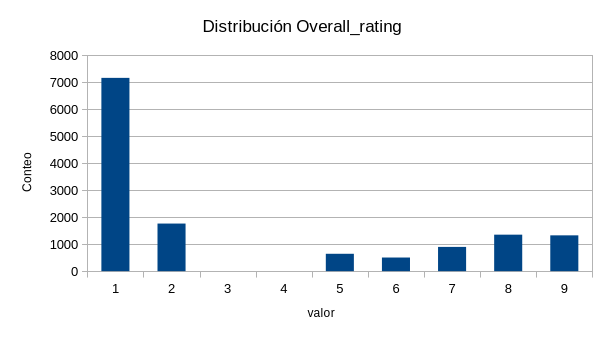
\includegraphics[width=0.85\linewidth]{distribucion_overall.png}\\
    \caption{Distribución de los valores de \textit{OVERALL\_RATING}.}
    \label{distribucion-overall}
\end{figure}

Se aprecia como se trata de un atributo con una distribución desigual, con
concentraciones en los valores extermos. Particularmente, la calificación 1 es
la más común con 7159 registros. Esto parece indicar un alto grado de
insatisfacción y un sesgo hacia las calificaciones negativas.
También es destacable la ausencia de reseñas con calificaciones intermedias (3 y
4).

Estos datos podrían ser problemáticos para el entrenamiento de modelos debido al
fuerte desbalanceo que existe entre clases.

\section{Preprocesado}
\label{chap:preprocess}
En este capítulo se describen las diferentes transformaciones aplicadas a los datos para su posterior uso en el entrenamiento de modelos.

\subsection{Transformación de \textit{OVERALL\_RATING} a nominal}
\label{sec:overalltransform}
Para poder construir un clasificador se ha transformado el atributo \textit{OVERALL\_RATING} de numérico a nominal; codificándolo en 3 clases:
\begin{itemize}
    \item 1: agrupa los valores comprendidos entre 1 y 3, ambos incluídos.
    \item 2: agrupa los valores comprendidos entre 4 y 6, ambos incluídos.
    \item 3: agrupo los valores comprendidos entre 7 y 9, ambos incluídos.
\end{itemize}

De esta forma también se trata de compensar la poca representación de algunos valores en el conjunto de datos. Cabe destacar que aun agrupando sigue habiendo una representación muy pobre de la clase \textit{2}.

\begin{table}[H]
    \begin{center}
        \begin{tabular}{@{}ccccc@{}}
            \toprule
            Clase                & 1              & 2      & 3\\
            \midrule
            Número de instancias & 8921           & 1148   & 3574 \\
            Porcentaje           & 65.39\%        & 8.41\% & 26.20\\
            \bottomrule
        \end{tabular}
        \caption{Porcentaje de representación de cada clase.}
    \end{center}
\end{table}

La sobrerrepresentación de la clase correspondiente a las evaluaciones más bajas se puede explicar a través de la tendencia de las personas a publicar una crítica en caso de descontento. A continuación se muestra un gráfico de tarta con la distribución de cada una de las clases:

\begin{figure}[H]
    \center
    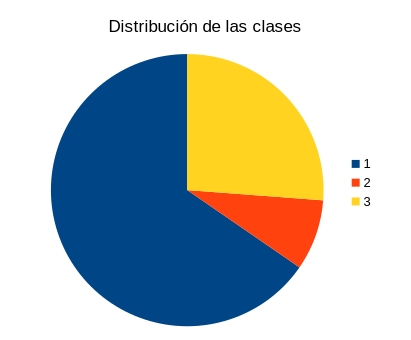
\includegraphics[width=0.60\linewidth]{overall_clases.png}\\
    \caption{Distribución de las clases.}
\end{figure}

\subsection{Eliminación de atributos}
\label{sec:delete_columns}
Se han seguido 3 criterios para la eliminación de atributos:
\begin{itemize}
    \item Relevancia: algunos datos no aportan información relevante de cara al entrenamiento del modelo. Por este criterio se han eliminado \textit{Date Flown} y \textit{Date Review}.
    \item Afectar negativamente al modelo: algunos atributos nominales cuentan con un número de clases muy numeroso. En el caso de \textit{Route}, tratar con todas ellas añade una gran complejidad que no se traduce a un mejor rendimiento. En consecuencia, se ha eliminado este atributo.
    \item Numerosos valores faltantes: se han eliminado todos los atributos con un número de \textit{missing values} superior al 35\% de los valores totales. Esto es porque se considera que no contamos con información suficiente para imputar estos datos.
\end{itemize}
A continuación se muestra un gráfico con el número de valores faltantes por atributo:

\begin{figure}[H]
    \center
    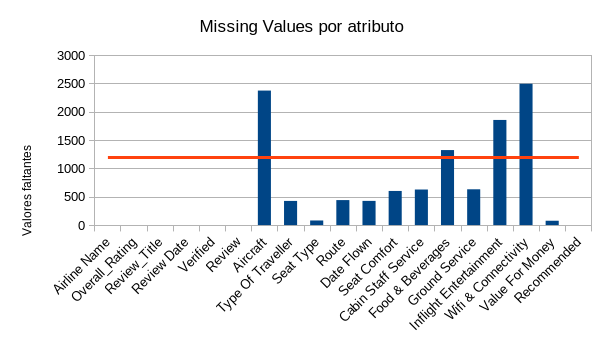
\includegraphics[width=0.85\linewidth]{missings.png}\\
    \caption{Número de valores faltantes por atributo.}
    \label{fig:missings}
\end{figure}

La línea sobre el gráfico \ref{fig:missings} señala el 35\% de las instancias. Por lo tanto, toda barra que rebase la línea se corresponde con un atributo a eliminar. Los atributos afectados han sido: \textit{Aircraft, Food \& Beverages, Inglight Entertainment} y \textit{Wifi \& Connectivity}.

\subsection{Formateo de los datos}
\label{sec:formateo}
Se han sustituído los valores de las columnas booleanas (i.e. \textit{Verified} y \textit{Recommended}) por valores binarios. Los valores nominales se han codificado mediante \textit{One-hot encoding}, a excepción de \textit{Airline} (esto es por limitaciones de la implementación). Los atributos codificados a través de \textit{OHE} han sido \textit{Seat Type} y \textit{Type of Traveller}.

\subsection{Imputación de valores faltantes}
\label{sec:imputacion}
En cuanto a la imputación de valores faltantes, se han reemplazado mediante el operador \textit{Replace Missing Values} de \textit{Altair AI Studio} por la moda de cada atributo. Los atributos afectados han sido \textit{Type Of Traveller, Seat Type, Food \& Bervarges, Groud Service, Seat Confort} y \textit{Value For Money}.

\section{Modelo básico sin usar datos textuales}
\label{chap:basicModel}
Se ha entrenado un modelo básico utilizando \textit{deep learning} para utilizarlo como referencia y cuantificar los beneficios proveídos por el \textit{text mining}. En la fase de preprocesado de los datos de este modelo solo se realiza la limpieza de datos relacionada con reemplazar datos faltantes y seleccionar atributos, eliminando todos los atributos de texto.

Se ha entrenado un modelo básico de \textit{deep learning} para utilizarlo como referencia y cuantificar los beneficios proveídos % paula en su momento de máxima inspiración lírica fdo. César
por el \textit{text mining}. Además del preprocesado de los datos especificado anteriormente, se han eliminando los atrbutos textuales \textit{Review} y \textit{Review Title}.

Tanto en el proceso de entrenamiento como en la evaluación se observa una \textit{accuracy} aproximada del 91\%. Se puede observar en la matriz de confusión que los resultados tanto de \textit{precission} como de \textit{recall} son muy buenos para las clases 1 y 3, siendo los valores en ambos casos cercanos al 90\%. Sin embargo, en el caso de la clase 2, estos los valores no alcanzan el 50\% de \textit{precission}. Concluímos que esto se debe a la poca representación de los datos de esta clase (8\%).

\section{Proceso de entrenamiento}
\label{chap:train}

En este capítulo se describen los procesos de entrenamiento para la construcción de los modelos de la parte 1 y parte 2. Para que el experimento sea reproducible se ha fijado una semilla a 1992 y se han marcado las opciones pertinentes en el software de \textit{Altair AI Studio} para la ejecución en un único hilo.

Cabe destacar que para la construcción de estos modelos se han empleado exclusivamente los atributos textuales \textit{Review} y \textit{Review Title}.

\subsection{Parte 1: Modelado sin análisis de sentimientos}
\label{sec:parte1}

    Para el entrenamiento de distintos modelos se ha trabajado con variaciones
    sobre los parámetros del preprocesado de los datos y los modelos usados.
    Además, se han empleado distintos tipos de modelo con sus
    parámetros por defecto con el fin de tener una mayor variedad y encontrar
    el más efectivo.

    De esta forma, se ha realizado un \textit{grid-search} con los siguientes valores:
    \begin{itemize}
        \item Preprocesado: \{\textit{TF-IDF}, \textit{Binary Term Occurrence}, \textit{prune below $3\%$}, \textit{prune below $10\%$}\}.
        \item Modelos: \{\textit{Deep Learning}, \textit{Random Forest}, \textit{Naive Bayes}, \textit{Decision Trees}\}
    \end{itemize}

    La función de evaluación de término determina qué se necesita para considerar
    que un término es relevante en un documento. Se han seleccionado ``TF-IDF'' y
    ``Binary Term Occurrence'' por representar 2 enfoques muy distintos. En el
    primer caso se necesita que el término sea muy frecuente en el documento pero
    muy poco frecuente en otros documentos, lo que puede significar que sea especialmente
    relevante en el documento. El segundo caso, sin embargo, es mucho más simple:
    únicamente comprueba si el término aparece en el documento o no.

    Con respecto al \textit{pruning}, hemos seleccionado una cota inferior del $3$ y $10$\%
    para eliminar los términos muy poco frecuentes según la función de evaluación
    de término. Se considera que estos términos no tendrán relevancia en los
    resultados, por lo que eliminarlos permitirá contruir modelos más simples y
    rápidos de entrenar sin cambiar los resultados. Inicialmente también se
    seleccionó una cota inferior del $0\%$, pero esto causó que hubiese demasiados
    términos en el resultado, incrementando demasiado el tiempo de ejecución del
    entrenamiento. Debido a esto, decidimos descartar este valor.

    Al concluir el entrenamiento se han obtenido los siguientes resultados:

    \footnotetext[1]{El formato de los parámetros es el siguiente: (\textit{Vector creation}, porcentaje de \textit{prune below}, modelo usado)}
    \begin{table}[H]
        \begin{center}
            \begin{tabular}{ @{}clc@{} }
                \toprule
                Modelo & Parámetros\footnotemark[1] & Accuracy\\
                \midrule
                1  & (\textit{TF-IDF}, $3\%$                 \textit{Deep Learning})  & $0.842 \pm 0.009$ \\
                2  & (\textit{TF-IDF}, $3\%$                 \textit{Random Forest})  & $0.660 \pm 0.006$ \\
                3  & (\textit{TF-IDF}, $3\%$                 \textit{Naive Bayes})    & $0.778 \pm 0.007$ \\
                4  & (\textit{TF-IDF}, $3\%$                 \textit{Decision Trees}) & $0.665 \pm 0.024$ \\
                5  & (\textit{Binary Term Occurrence}, $3\%$ \textit{Deep Learning})  & $0.843 \pm 0.005$ \\
                6  & (\textit{Binary Term Occurrence}, $3\%$ \textit{Random Forest})  & $0.805 \pm 0.010$ \\
                7  & (\textit{Binary Term Occurrence}, $3\%$ \textit{Naive Bayes})    & $0.748 \pm 0.009$ \\
                8  & (\textit{Binary Term Occurrence}, $3\%$ \textit{Decision Trees}) & $0.798 \pm 0.007$ \\
                9  & (\textit{TF-IDF}, $10\%$,               \textit{Deep Learning})  & $0.819 \pm 0.008$ \\
                10 & (\textit{TF-IDF}, $10\%$,               \textit{Random Forest})  & $0.743 \pm 0.009$ \\
                11 & (\textit{TF-IDF}, $10\%$,               \textit{Naive Bayes})    & $0.748 \pm 0.008$ \\
                12 & (\textit{TF-IDF}, $10\%$,               \textit{Decision Trees}) & $0.749 \pm 0.023$ \\
                \bottomrule
            \end{tabular}
            \caption{Parámetros y \textit{Accuracy} de los diferentes modelos -
            Parte 1.}
        \end{center}
    \end{table}

    \begin{figure}[H]
        \center
        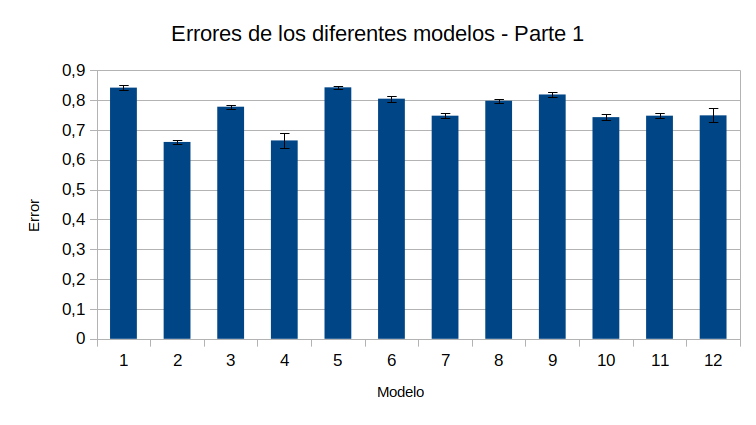
\includegraphics[width=0.85\linewidth]{errors_train1.png}\\
        \caption{\textit{Accuracy} de los diferentes modelos - Parte 1.}
    \end{figure}

    Al observar la comparación por pares proporcionada por el \textit{t-test},
    destacan el modelo 1 y 5 por obtener los mejores resultados y ser significativamente
    diferente de todos los demás. Ambos de estos modelos usan un \textit{prune below}
    del $3\%$ y ``Deep Learning''. El modelo 9 cuenta con el siguiente mejor error,
    aunque este es significativamente distinto del error de los modelos 1 y 5. Este
    modelo cuenta con un \textit{prune below} del $10\%$, lo cual puede eliminar
    demasiados términos, llegando a quitar términos potencialmente relevantes y
    explicando el peor rendimiento.

    Los modelos 1 y 5 se diferencian en la función de evaluación de término, pero
    esto no crea diferencias significativas en el error. En los tres casos la mejor
    familia de modelos es ``Deep Learning'', lo que indica que, en general, esta
    familia de modelos tiene una mejor capacidad para adaptarse a los datos y
    generalizar los patrones encontrados.

    Cabe destacar también que los modelos basados en ``Decision Trees'' obtienen
    una tolerancia en el error significativamente mayor que los demás modelos.
    Esto puede indicar que este tipo de modelos dependen mucho de los datos de
    entrenamiento usados, lo que puede dificultar la estimación de su rendimiento
    para nuevos datos.

    A continuación se muestra la matriz resultante de la ejecución del test:

    \begin{figure}[H]
        \center
        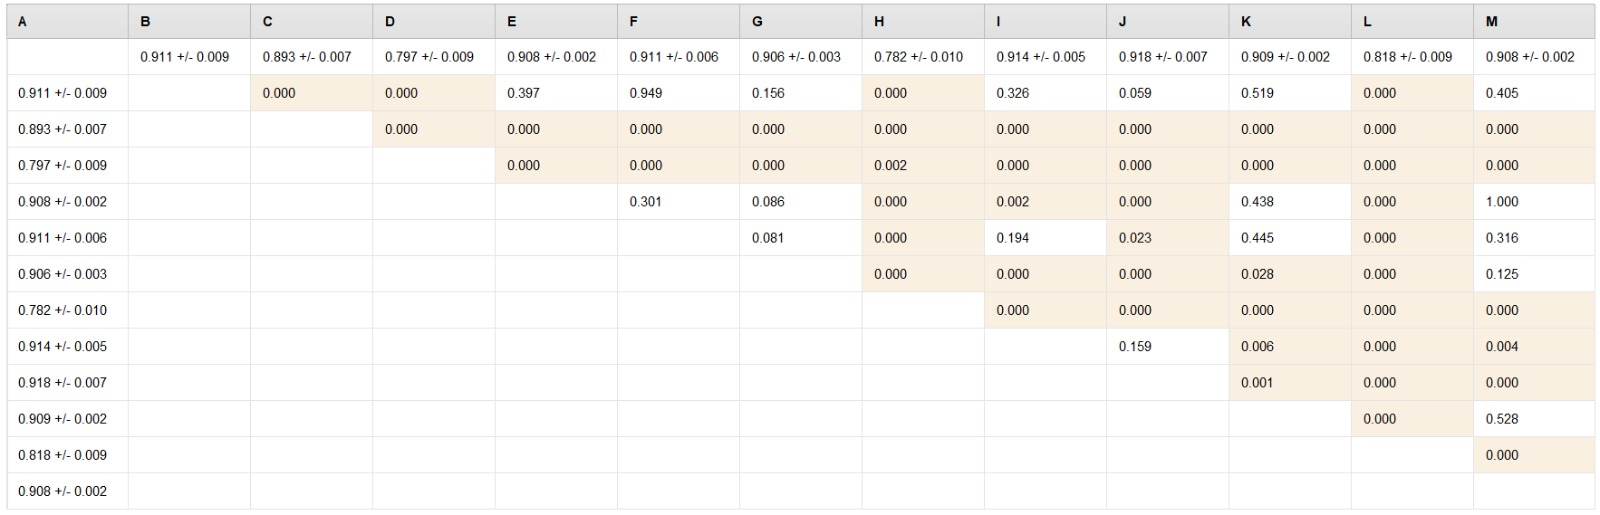
\includegraphics[width=\linewidth]{t_test1.jpeg}\\
        \caption{Resultado del \textit{t-test} de los modelos en el conjunto de
        \textit{train} - Parte 1.}
    \end{figure}

    Con toda esta información se concluye que el mejor modelo y con el que se hará
    la predicción es el modelo 4, debido a que es el modelo con mejor
    \textit{accuracy}, manteniendo una gran simplicidad al usar \textit{Binary Term
    Occurrence}. En la siguiente figura se muestra el \textit{recall} y
    \textit{precision} de las diferentes clases para este modelo.

%    \begin{figure}[H]
%        \center
%        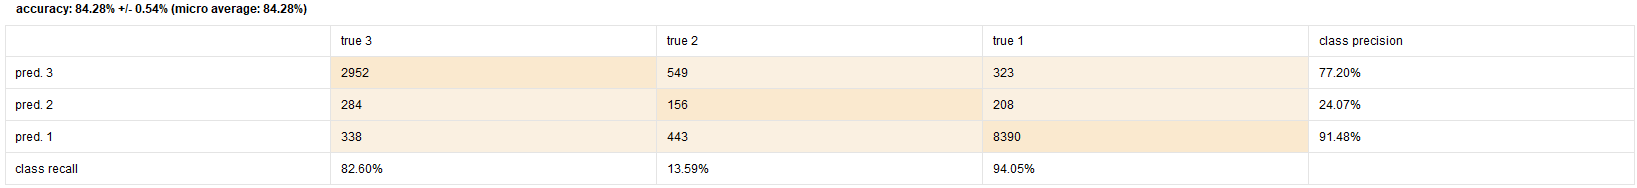
\includegraphics[width=\linewidth]{train1.jpeg}\\
%        \caption{Precision y recall del modelo 9 en el conjunto de
%        \textit{train} - Parte 1.}
%    \end{figure}
\begin{table}[H]
\center
\begin{tabular}{@{}lccc|c@{}}
    \toprule
             & True 3 & True 2 & True 1 & precision\\
    \hline
    pred. 3  & 2952   & 549    & 323    & 0.7720   \\
    pred. 2  & 284    & 156    & 208    & 0.2407   \\
    predl 1  & 338    & 443    & 8390   & 0.9148   \\
    \hline
    recall   & 0.8260 & 0.1359 & 0.9405 &          \\
    \bottomrule
\end{tabular}
\caption{Matriz de confusión del modelo 9 en el conjunto de \textit{train} -
parte 1.}
\end{table}

\subsection{Parte 2: Modelado con análisis de sentimientos}
\label{sec:parte2}

    Al igual que en la parte anterior, se ha trabajado con variaciones
    sobre los parámetros del preprocesado de los datos y los modelos usados.

    De esta forma se realiza un \textit{grid-search} con los siguientes valores:
    \begin{itemize}
        \item Preprocesado: \{\textit{bigramas}, \textit{trigramas}, \textit{prune below $3\%$}, \textit{prune below $10\%$}\}.
        \item Modelos: \{\textit{Deep Learning}, \textit{Random Forest}, \textit{Naive Bayes}, \textit{Decision Trees}\}
    \end{itemize}

    La longitud de los n-gramas permite reconocer términos compuestos por múltiples
    palabras, pero si es demasiado grande puede generar muchos términos sin significado
    semántico. Hemos seleccionado longitudes de $2$ y $3$ ya que permite reconocer
    la mayoría de términos compuestos sin permitir generar términos compuestos
    por demasiadas palabras.

    Con respecto al \textit{pruning}, hemos seleccionado una cota inferior del $3$ y $10$\%
    para eliminar los términos sin significado semántico que pueden generar los
    n-gramas. Estos términos serán muy poco frecuentes en los datos, por lo que
    estarán por debajo de esta cota inferior. Inicialmente también se seleccionó
    una cota inferior del $0\%$, pero esto causó que hubiese demasiados términos
    en el resultado, incrementando en gran el tiempo de ejecución del entrenamiento, sin que esto se tradujera a un mejor rendimiento.
    Debido a esto, decidimos descartar este valor.

    Al concluir el entrenamiento se han obtenido los siguientes resultados:

    \footnotetext[2]{El formato de los parámetros es el siguiente: (Longitud $n$-gramas, porcentaje de \textit{prune below}, modelo usado)}
    \begin{table}[H]
        \begin{center}
            \begin{tabular}{ @{}clc@{} }
                \toprule
                Modelo & Parámetros\footnotemark[2] & Accuracy\\
                \midrule
                1  & (\textit{Bigramas},  $3\%$, \textit{Deep Learning})  & $0.845 \pm 0.007$ \\
                2  & (\textit{Bigramas},  $3\%$, \textit{Random Forest})  & $0.655 \pm 0.001$ \\
                3  & (\textit{Bigramas},  $3\%$, \textit{Naive Bayes})    & $0.784 \pm 0.007$ \\
                4  & (\textit{Bigramas},  $3\%$, \textit{Decision Trees}) & $0.669 \pm 0.024$ \\
                5  & (\textit{Trigramas}, $3\%$, \textit{Deep Learning})  & $0.847 \pm 0.006$ \\
                6  & (\textit{Trigramas}, $3\%$, \textit{Random Forest})  & $0.656 \pm 0.003$ \\
                7  & (\textit{Trigramas}, $3\%$, \textit{Naive Bayes})    & $0.784 \pm 0.007$ \\
                8  & (\textit{Trigramas}, $3\%$, \textit{Decision Trees}) & $0.670 \pm 0.025$ \\
                9  & (\textit{Bigramas}, $10\%$, \textit{Deep Learning})  & $0.815 \pm 0.007$ \\
                10 & (\textit{Bigramas}, $10\%$, \textit{Random Forest})  & $0.730 \pm 0.015$ \\
                11 & (\textit{Bigramas}, $10\%$, \textit{Naive Bayes})    & $0.761 \pm 0.010$ \\
                12 & (\textit{Bigramas}, $10\%$, \textit{Decision Trees}) & $0.752 \pm 0.038$ \\
                \bottomrule
            \end{tabular}
            \caption{Parámetros y \textit{Accuracy} de los diferentes modelos -
            Parte 2.}
        \end{center}
    \end{table}

    \begin{figure}[H]
        \center
        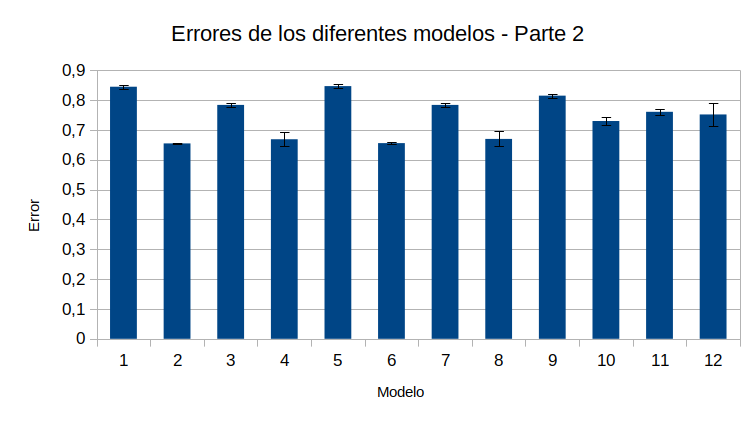
\includegraphics[width=0.85\linewidth]{errors_train2.png}\\
        \caption{\textit{Accuracy} de los diferentes modelos - Parte 2.}
    \end{figure}

    Al observar la comparación por pares proporcionada por el \textit{t-test},
    destacan de nuevo el modelo 1 y 5 (\textit{Deep Learning}
    con \textit{prune below $3\%$}). De la misma forma que en la parte anterior,
    el siguiente modelo con el mejor error es el 9 (\textit{prune below $10\%$}),
    verificando la hipótesis realizada anteriormente de que este valor de
    \textit{prune below} es demasiado alto y elimina términos relevantes. Además,
    ambos de los modelos con el mejor error usan la familia de modelos de
    ``Deep Learning'', confirmando también la hipótesis de que esta familia tiene
    una mejor capacidad de aprendizaje y generalización. Por último, también se
    puede ver que los modelos basados en ``Decision Trees'' siguen teniendo una
    tolerancia en el error significativamente más alta que los demás modelos,
    confirmando la hipótesis de que estos modelos dependen mucho de los datos
    utilizados para el entrenamiento.

    En este caso, la diferencia entre los modelos 1 y 5 es la longitud de los
    n-gramas usados. Como no hay diferencias significativas en los errores de
    estos modelos, se puede concluir que no hay n-gramas de longitud 3
    relevantes en los datos.

    A continuación se muestra la matriz resultante de la ejecución del test:

    \begin{figure}[H]
        \center
        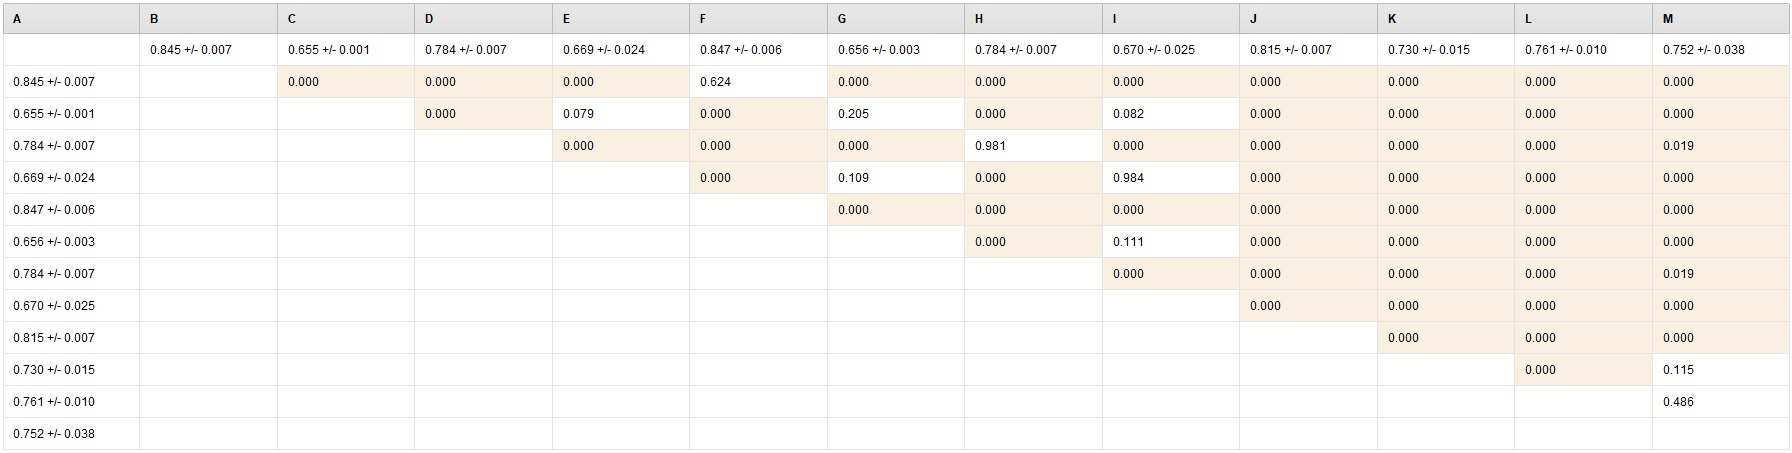
\includegraphics[width=\linewidth]{t_test2.jpg}\\
        \caption{Resultado del \textit{t-test} de los modelos en el conjunto de
        \textit{train} - Parte 2.}
    \end{figure}

    Con toda esta información se concluye que el mejor modelo y con el que se
    hará la predicción es el modelo 1, debido a que es el modelo con mejor
    \textit{accuracy} y es de los modelos más simples al usar \textit{bigramas}.
    En la siguiente figura se muestra el \textit{recall} y \textit{precision} de
    las diferentes clases para este modelo.

%    \begin{figure}[H]
%        \center
%        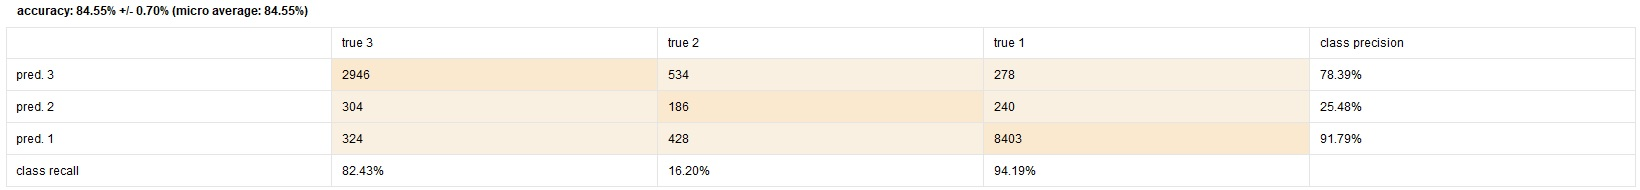
\includegraphics[width=\linewidth]{train2.jpeg}\\
%        \caption{Precision y recall del modelo 9 en el conjunto de
%        \textit{train} - Parte 2.}
%    \end{figure}
\begin{table}[H]
\center
\begin{tabular}{@{}lccc|c@{}}
    \toprule
             & True 3 & True 2 & True 1 & precision\\
    \hline
    pred. 3  & 2946   & 534    & 278    & 0.7839   \\
    pred. 2  & 304    & 186    & 240    & 0.2548   \\
    predl 1  & 324    & 428    & 8403   & 0.9179   \\
    \hline
    recall   & 0.8243 & 0.1620 & 0.9419 &          \\
    \bottomrule
\end{tabular}
\caption{Matriz de confusión del modelo 9 en el conjunto de \textit{train} -
parte 2.}
\end{table}


\section{Comparación de resultados}
\label{chap:resultados}

En este capítulo se comparan los resultados obtenidos en los diferentes procesos para cada uno de los modelos.

\subsection{Procesos de entrenamiento}
\label{subsec:comparar_train}
Durante el proceso de entrenamiento destaca positivamente el modelo base,
contando con un \textit{Accuracy} superior al $91\%$. Los modelos basados en
\textit{minería de texto} cuentan con un rendimiento muy similar, entorno al
$84\%$. Es relevante mencionar que la clase mejor predicha en todos los modelos
es la clase 1, hecho que se explica por la sobrerrepresentación de esta clase en
el conjunto de los datos. En contraste, la clase con la puntuación más baja es
la clase 2. A continuación se muestra una tabla y un gráfico que recogen el
\textit{Accuracy} por cada clase y modelo.
\begin{table}[H]
\center
\begin{tabular}{@{}lccc@{}}
    \toprule
    modelo      & acc. clase1&	acc. clase2	& acc. clase 3 \\
    \midrule     
    modelo base & 0.9741 & 0.4199	& 0.9387 \\
    modelo p1   & 0.9405 & 0.1359	& 0.826 \\
    modelo p2   & 0.9419 & 0.162	& 0.824 \\
    \bottomrule
\end{tabular}
    \caption{Accuracy por modelo y clase en el conjunto de entrenamiento.}
\end{table}
\begin{figure}[H]
    \center
    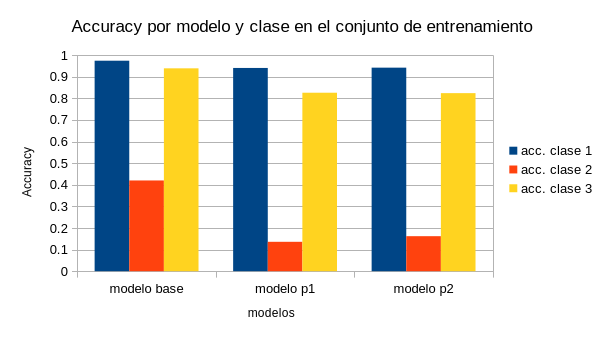
\includegraphics[width=0.85\linewidth]{accModClassTrain.png}\\
    \caption{Accuracy por modelo y clase en el conjunto de \textit{train}.}
\end{figure}

Tal y como se esperaba en un inicio, las clases mejor predichas son aquellas con
un mayor número de instancias. Cabe destacar el rendimiento superior del modelo
base, especialmente hablando de la clase 2. Estos resultados parecen indicar que
los campos textuales no contienen suficiente información para distinguir las
reseñas intermedias (clase 2) de las de otro tipo.

Al observar a la matriz de confusión, de cada modelo
se aprecia como los valores de \textit{precision} y \textit{recall} son
similares para las clases 1 y 3 en todos los modelos. Esto parece indicar que se
tratan de modelos robutos que son capaces de capturar y clasificar correctamente
todas las instancias de estas clases. Para la clase 2, los valores de \textit{precision} y \textit{recall} son
similares únicamente en el caso del modelo base. Para los demás modelos, estos
valores son muy bajos y desbalanceados hacia la \textit{precision}. En cualquier
caso, las medidas realizadas sobre la clase 2 para todos los modelos indican que
ninguno ha sido capaz de capturar y clasificar correctamente las instancias de
esta clase; muy probablmente debido a la poca representación de la misma en el
conjunto de los datos.

\subsection{Evaluación}
\label{subsec:comparar_test}

Tras realizar predicciones sobre el conjunto de \textit{test} los resultados
obtenidos con cada modelo han sido los siguientes:

\begin{table}[H]
\center
\begin{tabular}{@{}lccc@{}}
    \toprule
    modelo      & acc. clase1&	acc. clase2	& acc. clase 3 \\
    \midrule     
    modelo base & 0.9837     & 0.4184	& 0.8896 \\
    modelo p1   & 0.9851     & 0.0	    & 0.7038 \\
    modelo p2   & 0.9435     & 0.2163	& 0.7934 \\
    \bottomrule
\end{tabular}
    \caption{Accuracy por modelo y clase en el conjunto de test.}
\end{table}
\begin{figure}[H]
    \center
    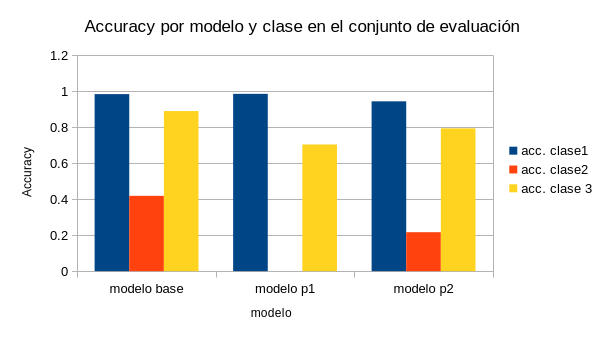
\includegraphics[width=0.85\linewidth]{accModClassTest.png}\\
    \caption{Accyracy por modelo y clase en el conjunto de test.}
\end{figure}

Se aprecia un comportamiento similar de los modelos al compararlos con los
resultaods obtenidos en el entrenamiento. Esto significa que ninguno de los
modelos ha sufrido de \textit{overfitting}. Destaca que el modelo de la parte 1
no ha sido capaz de predecir correctamente ninguna de las instancias de la clase
2. También es notable cómo el modelo base cuenta con un rendimiento superior al
resto de modelos. Los modelos de la parte 1 y parte 2 se comportan de forma
similar, destacando el segundo por mostrar un mejor rendimiento en para las
clases minoritarias.

A continuación, con el fin de hacer un análisis más profundo, se desglosarán las
predicciones en una matriz de confusión para cada modelo.

\subsubsection{Modelo base}
\label{eva-modelobase}
La matriz correspondiente al modelo base, construído exclusivamente con
atributos no textuales, es la siguiente:

\begin{table}[H]
\center
\begin{tabular}{@{}lccc|c@{}}
    \toprule
             & True 3 & True 2 & True 1 & precision\\
    \hline
    pred. 3  & 814   & 75      & 4      & 0.9115   \\
    pred. 2  & 88    & 118     & 32     & 0.4958   \\
    predl 1  & 13    & 89      & 2178   & 0.9553   \\
    \hline
    recall   & 0.8896 & 0.4184 & 0.9837 &          \\
    \bottomrule
\end{tabular}
\caption{Matriz de confusión del modelo base con el conjunto \textit{test}.}
\end{table}

Se aprecia que las medidas para \textit{precision} y \textit{recall} son altas y
similares para las clases mayoritarias. Lo que significa que se trata de un modelo robusto capaz de capturar
y predecir correctamente las instancias pertenencientes a las clases 1 y 3. Para
la clase 2, contamos con las medidas más altas entre los 3 modelos. No obstante,
siguen siendo medidas muy bajas que muestran un rendimiento pobre para esta
clase de instancias. Cabe destacar que el modelo clasifica una cantidad mayor de
instancias de la clase 3 como clase 2. Esto indica que existe una separación más
clara entre las instancias de la clase 1 y la clase 2 que entre la clase 3 y la
clase 2. Esto se puede corroborar comprobando la distribución de los valores de la variable
objetivo \textit{OVERALL\_RATING} previo a la transformación del atributo de
numérico a nominal (figura~\ref{distribucion-overall}).

\subsubsection{Parte 1: modelo con \textit{text mining}}
\label{eva-modeloparte1}
La matriz correspondiente al modelo de la parte 1, construído con atributos
exclusivamente textuales y sin uso de análisis de sentimientos, es la siguiente:

\begin{table}[H]
\center
\begin{tabular}{@{}lccc|c@{}}
    \toprule
             & True 3 & True 2 & True 1 & precision\\
    \hline
    pred. 3  & 644 & 105       & 33     & 0.8235   \\
    pred. 2  & 3   & 0         & 0      & 0.0      \\
    predl 1  & 268 & 177       & 2181   & 0.8305   \\
    \hline
    recall   & 0.9851 & 0.0 & 0.7038 &          \\
    \bottomrule
\end{tabular}
\caption{Matriz de confusión del modelo de la parte 1 con el conjunto \textit{test}.}
\end{table}

Este modelo emplea técnicas de \textit{text mining} para analizar los campos
\textit{Review} y \textit{Review title} y una red neuronal (operador
\textit{DeepLearning}~\cite{deeplearning} del software). 

De forma similar al modelo anterior, las medidas de \textit{precision} y
\textit{recall} son altas y similares para las clases mayoritarias. De nuevo, se
trata de un modelo robusto capaz de reconocer y clasificar correctamente las
instancias pertenencientes a las clases mayoritarias. El modelo muestra un
rendimiento notablemente superior en la clasificación de instancias de la clase
1, hecho esperable ya que se trata de la clase mayoritaria. Sin embargo, muestra un
rendimiento paupérrimo para la clase 2, seguramente debido a la poca
representación de esta clase. El modelo no ha sido capaz de capturar ninguna de
las 282 instancias de la esta clase.

\subsubsection{Parte 2: modelo con \textit{text mining}, \textit{sentiment
analysis} y \textit{n-gramas}}
\label{eva-modeloparte2}

La matriz correspondiente al modelo de la parte 2, construído con atributos
exclusivamente textuales y empleando análisis de sentimientos y construcción de
n-gramas, es la siguiente:

\begin{table}[H]
\center
\begin{tabular}{@{}lccc|c@{}}
    \toprule
             & True 3 & True 2 & True 1 & precision\\
    \hline
    pred. 3  & 644 & 105       & 33     & 0.8235   \\
    pred. 2  & 3   & 0         & 0      & 0.0      \\
    predl 1  & 268 & 177       & 2181   & 0.8305   \\
    \hline
    recall   & 0.9851 & 0.0 & 0.7038 &          \\
    \bottomrule
\end{tabular}
\caption{Matriz de confusión del modelo de la parte 1 con el conjunto \textit{test}.}
\end{table}

Este modelo emplea técnicas de \textit{text mining} para analizar los campos
\textit{Review} y \textit{Review title}. Además, realiza un análisis de
sentimientos y construye n-gramas de tamaño 2. Por último, emplea una red neuronal (operador
\textit{DeepLearning}~\cite{deeplearning} del software) para realizar la
predicción.

Al igual que en los anteriores modelos, las medidas de \textit{precision} y
\textit{recall} son altas y similares para las clases mayoritarias; demostrando
ser un modelo robusto para las clases 1 y 3. El modelo muestra un
rendimiento significativamente superior en la clasificación de instancias de la clase
2 al compararlo con el modelo 1, lo que parece demostrar que el analisis de
sentimientos y la construccion de bigramas permiten reconocer nuevos patrones
capaces de separar las instancias de la clase 2. Sin embargo, el rendimiento
para esta clase sigue siendo muy bajo, mostrando como el conjunto de datos no
cuenta con representación suficiente de esta clase como para construir un modelo capaz de
predecir correctamente este tipo de instancias.

\subsection{Conclusiones de los resultados}
\label{subsec:comparar_conclusiones}

Los tres modelos predicen correctamente las instancias pertenecientes a las
clases mayoritarias. Destacando el modelo base al mostrar mejor rendimiento para
ambas clases. Sin embargo, cabe destacar que los modelos basados en
\textit{text mining} han empleado únicamente 2 atributos del conjunto de datos.

También se aprecia que, pese a que el modelo de la parte 1 tenga un mejor
rendimiento para la clase 1, el análisis de sentimientos y la construcción de
n-gramas hacen que el modelo de la parte 2 tenga un mejor rendimiento general.

En cuanto a la clase 2, ninguno de los modelos ha logrado tener un rendimiento
suficiente en el reconocimiento de este tipo de instancias. Siendo el que
mejores resultados presenta el modelo base. Destaca que el modelo de la parte 2
es capaz de capturar más instancias que el modelo de la parte 1, por lo que se
concluye que el análisis de sentimientos permite segregar mejor el conjunto de
los datos.

Con todo lo anterior, se concluye que en el conjunto de datos existe suficiente
información en los atributos no textuales para la construcción de modelos
robustos de clasificación. Sin embargo, las técnicas de \textit{text mining} y
análisis de sentimientos han demostrado ser muy potentes y capaces de reconocer
patrones y extraer información a partir de menos atributos; logrando acercarse
al rendimiento del modelo base. Es importante mencionar que para la construcción
de un modelo capaz de trabajar con las instancias de la clase 2 se proponen 3
alternativas:

\begin{itemize}
    \item Mayor recopilación de datos de estas instnacias: recoger más datos de
    reseñas con puntuaciones entre 3 y 6.
    \item Utilización de técnicas de \textit{Undersampling} de las clases
    mayoritarias: especialmente de la clase 1.
    \item Otras divisiones de los datos: se podría trabajar con 2 clases en
    lugar de 3, agrupando la clase 2 y la clase 3 en una única clase. Sin
    embargo, seguiría existiendo un desbalanceo hacia la clase 1.
    automático.
\end{itemize}

\section{Parte opcional: Topic modelling}
\label{chap:topic}

Se ha realizado un último análisis de los datos como parte de la sección
opcional de la investigación basado en el \textit{topic} modelling. El objetivo de este
es identificar patrones en los datos que puedan agrupar las reseñas en
distintos grupos. Para esto se va a utilizar el operador de RapidMiner “Extract
Topics from Data”, que usa el algoritmo de Latent Dirichlet Allocation para
identificar y agrupar temas de los documentos.

El preprocesado de los datos para la aplicación de este algoritmo será similar
al utilizado en las dos partes anteriores de este trabajo, con la excepción de
la eliminación del atributo objetivo. Este preprocesado es realizado para poder
comparar los resultados con los datos de manera efectiva, aunque en el operador
solo se utilice la columna “Review”. Se buscará agrupar las reseñas de dos
maneras modificando el parámetro \textit{number of topics}:

\begin{itemize}
    \item En dos grupos, con la hipótesis de que se dividirán en positivas y
    negativas. En este caso se compararán los grupos obtenidos con la columna
    de \textit{Recommended}, considerándose esta una buena medida de la positividad
    de la reseña.
    \item En tres grupos que se compararán con el valor de \textit{OVERALL\_RATING} ya
    reducido a tres opciones en el preprocesado. El objetivo es comprobar si
    estos textos cuentan con agrupaciones naturales que se relacionen con la
    valoración final del usuario.
\end{itemize}

Además, en ambos casos se comprobarán las \textit{top words} proporcionadas por cada
una de las agrupaciones con el objetivo de identificar los temas obtenidos.
Cabe resaltar que se utilizará la opción de 10 \textit{top words} por ser este un número
lo suficientemente grande como para recabar información aún siendo manualmente
analizable. Este parámetro no afecta al agrupamiento final o al rendimiento del
proceso.

Se van a utilizar 1000 iteraciones para ambos procesos, siendo este un número
que consigue una buena precisión en los resultados sin sacrificar el
rendimiento. Se han explorado rangos más bajos y más altos de iteraciones, sin
éxito. En el primer caso la reducción de precisión era demasiado
significativa y en el segundo el aumento del tiempo no llevaba a una mejora
sustancial.

Con estos parámetros se han obtenido los resultados expuestos a continuación.

\subsection{Generación de 2 grupos y comparación con \textit{Recommended}}
\label{subsec:topicmodelling-recommended}

Una vez ejecutado el modelo se consiguen dos salidas: las instancias
clasificadas en dos grupos distintos y las 10 palabras más comunes en ambos
grupos. Las instancias clasificadas han sido comparadas con su valor en el
atributo “Recommended”, obteniendo el siguiente resultado:

\begin{table}[H]
\center
\begin{tabular}{@{}cccc@{}}
    \toprule
    TopicID & Nº Instancias & Recommended = 0 & Recommended = 1 \\
    \midrule
    0       & 8216          & 7949            & 367 \\
    1       & 5327          & 1603            & 3724\\
    \bottomrule
\end{tabular}
\caption{Resultados de topic modelling basado en Recommended.}
\end{table}

\begin{figure}[H]
    \center
    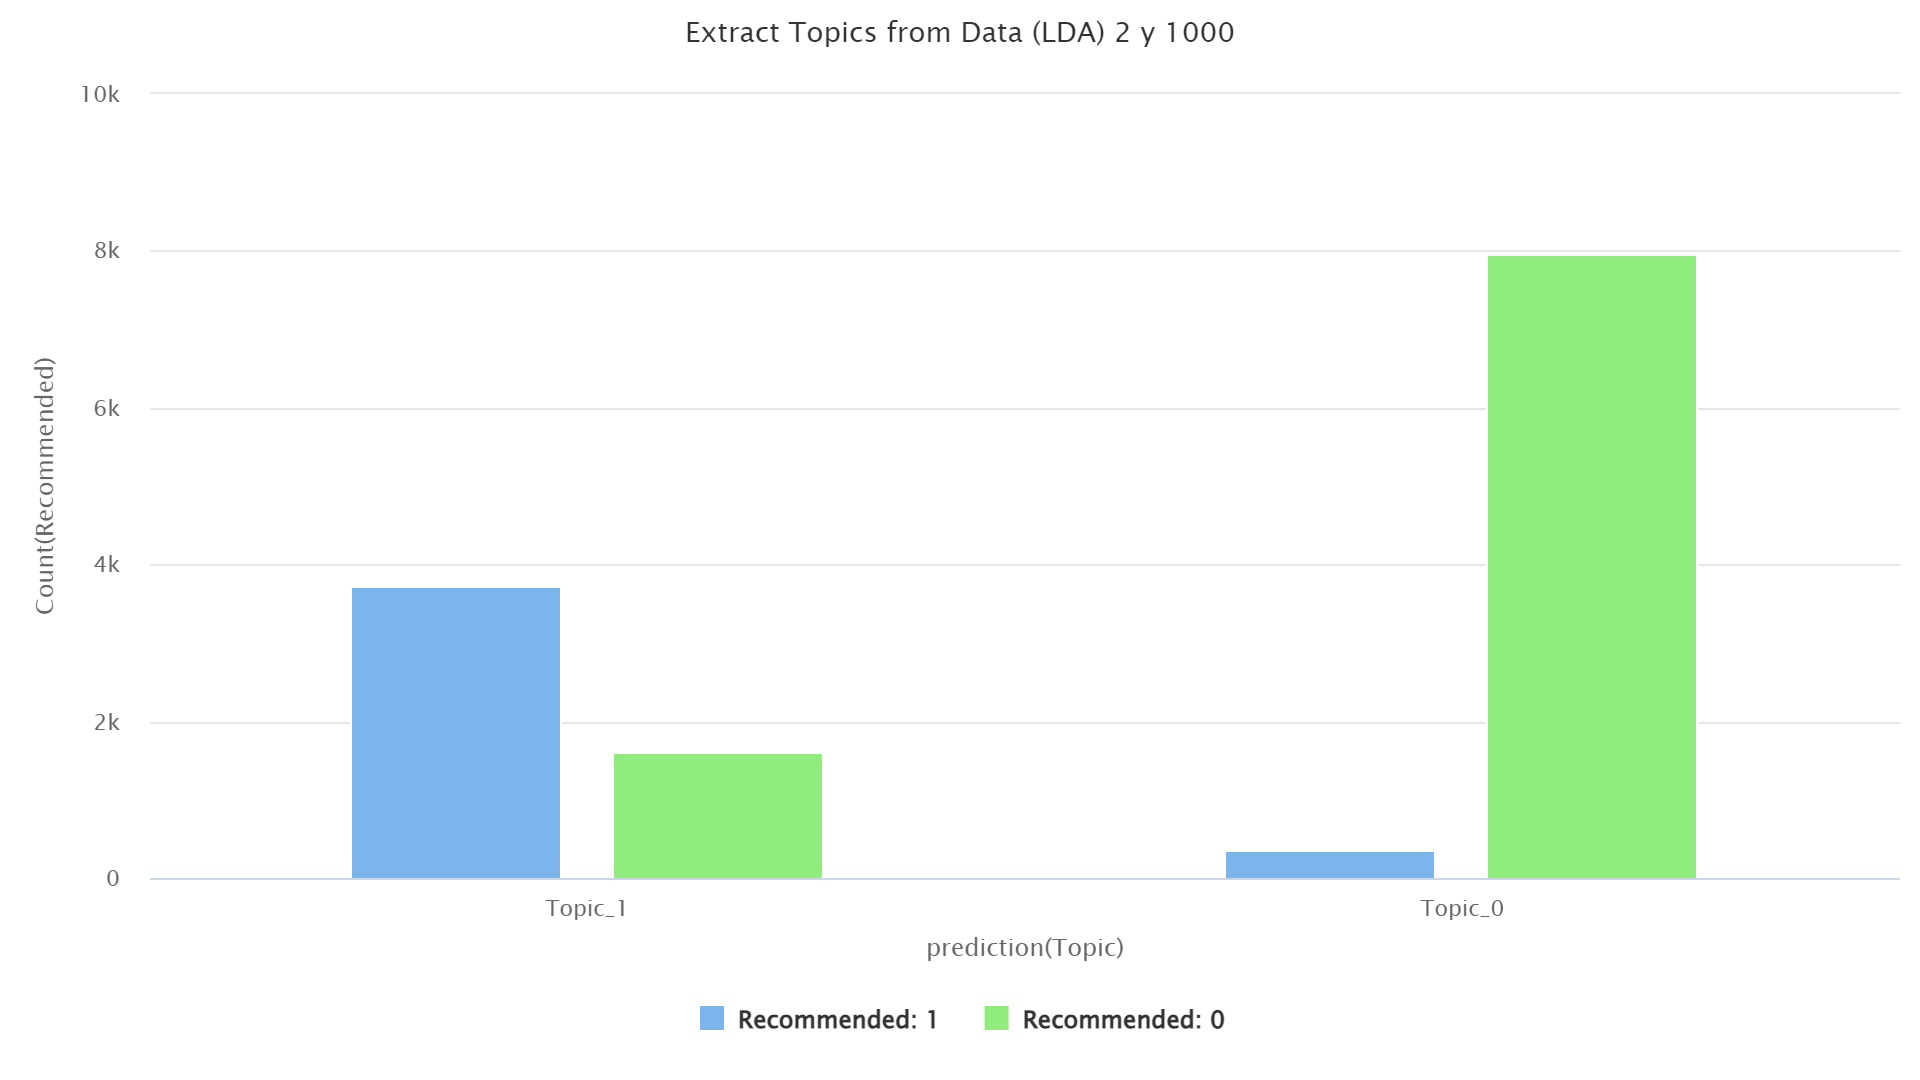
\includegraphics[width=0.85\linewidth]{graph_2topic_1000iter_other.jpeg}\\
    \caption{Resultados de topic modelling basado en Recommended.}
\end{figure}

Se puede observar que ambos grupos cuentan con una mayoría de instancias de una
de las categorías de “Recommended”, lo cual puede indicar que las agrupaciones
corresponden en cierta medida con la opinión general de los usuarios. En el
caso del grupo 0 la diferencia parece mucho menor, pero esto probablemente esté
causado por el desbalance que existe en las clases de “Recommended”, siendo la
clase 0 casi tres veces más común que la 1. Así, se puede concluir que la
clasificación en grupos del LDA es correcta en relación con este atributo.

Al analizar las palabras más comunes de ambas agrupaciones se pueden encontrar
nombres y adjetivos que pueden apoyar la idea de que efectivamente se han
creado dos grupos de experiencias positivas y negativas.

\begin{table}[H]
    \center
    \begin{tabular}{@{}ccc@{}}
        \toprule
        topicid & word & weight \\
        \midrule
        0 & flight  & 17165 \\
        0 & airline & 6157  \\
        0 & hours   & 4662  \\
        0 & get     & 4303  \\
        0 & time    & 4248  \\
        0 & airport & 4090  \\
        0 & service & 4083  \\
        0 & would   & 4075  \\
        0 & told    & 3723  \\
        0 & one     & 3280  \\
        \bottomrule
    \end{tabular}
    \hspace{2.5mm}
    \begin{tabular}{@{}ccc@{}}
        \toprule
        topicid & word & weight \\
        \midrule
        1 & flight  & 7211  \\
        1 & good    & 3358  \\
        1 & time    & 2970  \\
        1 & crew    & 2955  \\
        1 & seats   & 2907  \\
        1 & service & 2842  \\
        1 & seat    & 2773  \\
        1 & food    & 2629  \\
        1 & cabin   & 2237  \\
        1 & staff   & 1862  \\
        \bottomrule
    \end{tabular}
    \caption{Top words en las agrupaciones por Recommended.}
\end{table}

En el grupo 0, que corresponde a las experiencias negativas, se encuentran
palabras como ``hours'' que probablemente tengan relación con malas experiencias
de tiempos de espera o cancelaciones. En el segundo grupo, sin embargo, se
encuentran palabras como ``good'' o ``staff'' que representan opiniones positivas
sobre el vuelo y los empleados. Cabe destacar que aunque existan palabras
útiles para el análisis en ambos casos, la mayoría de palabras son comunes
entre ambos grupos y no cuentan con una connotación negativa o positiva, siendo
inútiles para conseguir conclusiones. Especialmente, ``flight'' o ``time'' dependen
completamente del calificativo del que van acompañadas, por lo que sería
necesario realizar un análisis que permita expresiones de varias palabras.

\subsection{Generación de 3 grupos y comparación con \textit{Overall\_Rating}}

En la segunda aproximación los resultados de la clasificación son:

\begin{table}[H]
\center
\begin{tabular}{@{}ccccc@{}}
    \toprule
    TopicID & Nº Instancias & Overall Rating = 1 & Overall Rating = 2 & Overall Rating = 3 \\
    \midrule
    0       & 5281          & 4762               & 230                & 289 \\
    1       & 3354          & 3196               & 73                 & 85  \\
    2       & 5008          & 963                & 845                & 3200\\
    \bottomrule
\end{tabular}
\caption{Resultados de topic modelling basado en Overall\_Rating.}
\end{table}

\begin{figure}[H]
    \center
    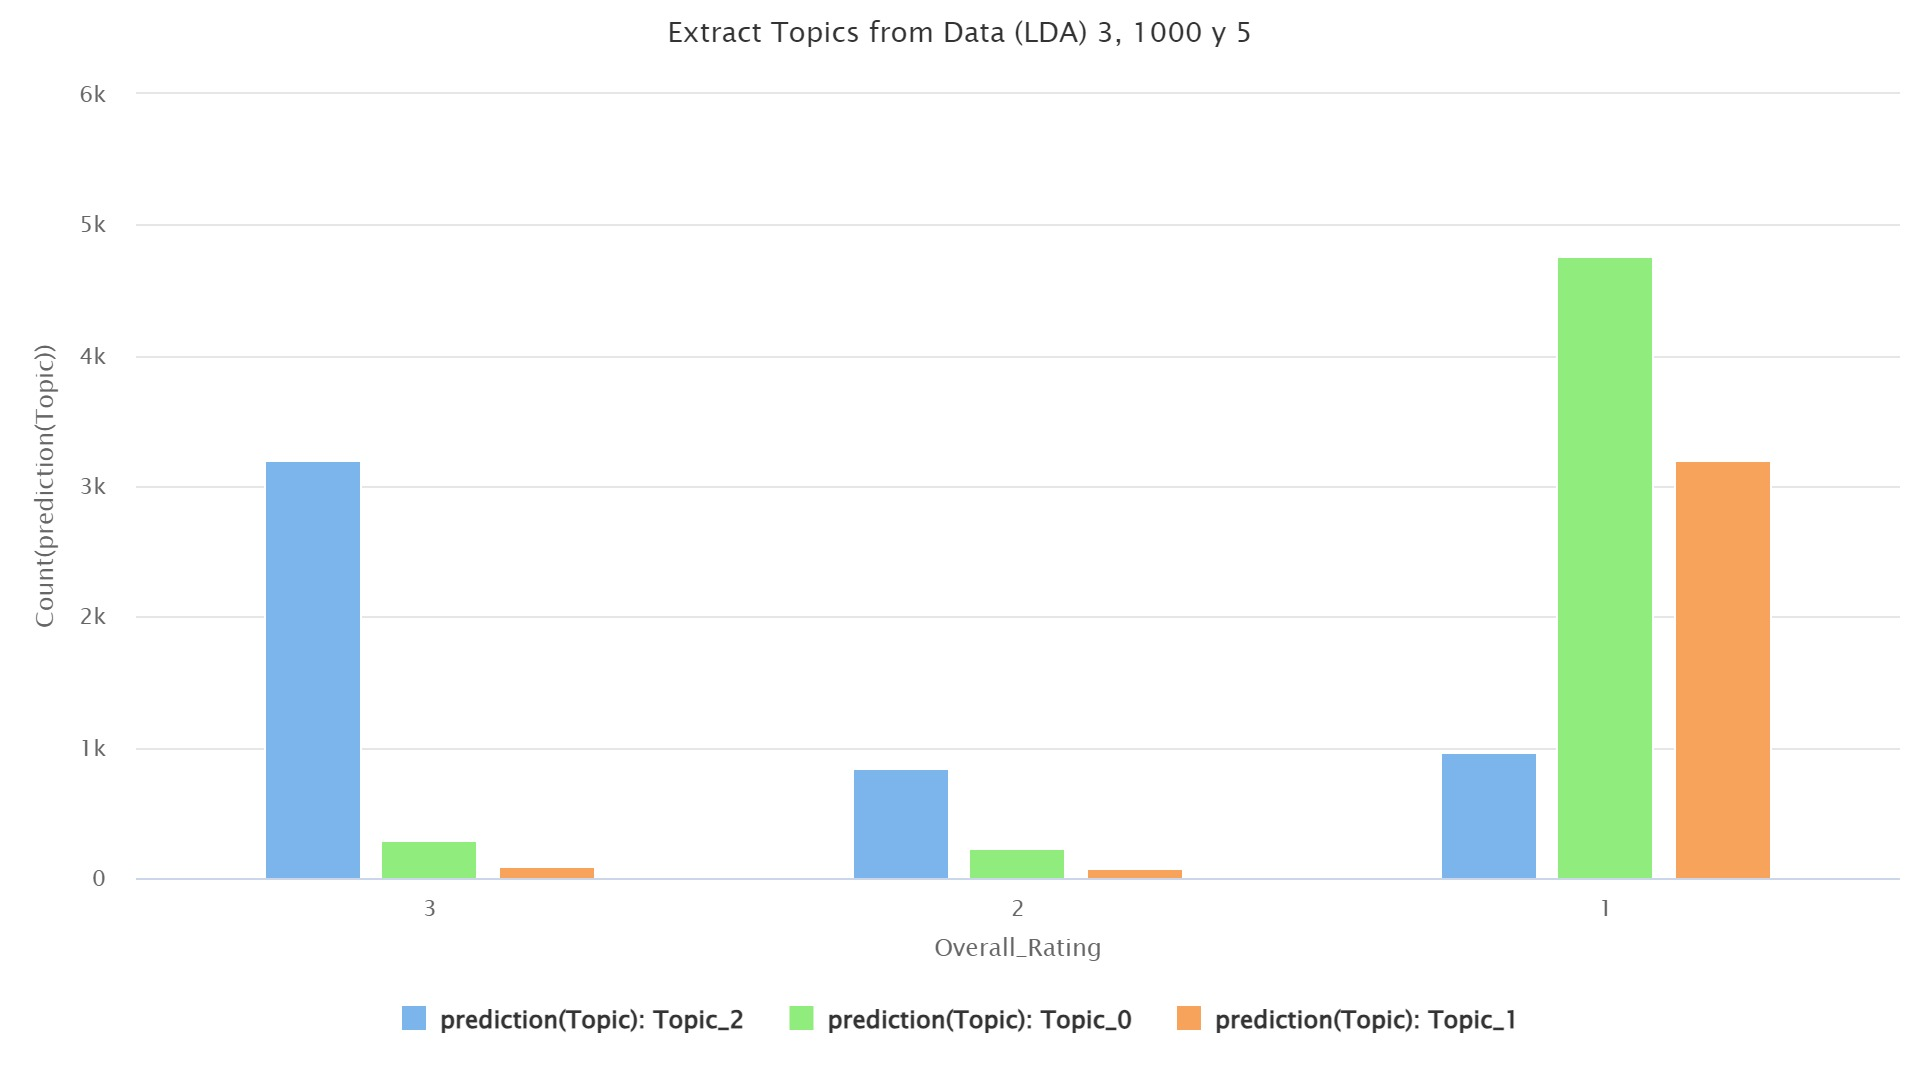
\includegraphics[width=0.85\linewidth]{graph_3topic_1000iter.jpeg}\\
    \caption{Resultados de topic modelling basado en Overall\_Rating.}
\end{figure}

Una vez más se observa que el desbalance de las clases del atributo provoca una
diferencia en la precisión de los resultados entre los grupos. En este caso,
aunque el \textit{topic} 2 representa de manera significativa las valoraciones positivas
de los usuarios, los \textit{topics} 0 y 1 parecen ambos corresponder con las instancias
negativas. La poca existencia de instancias que representen la clase 2 de
Overall Rating probablemente se corresponde con la falta de existencia de una
agrupación natural de los datos para esta. Así, se puede teorizar que solo
existen dos agrupaciones de datos, siendo el grupo intermedio insignificante.
Esta teoría viene además acompañada de los datos de las \textit{top words} de cada
agrupación:

\begin{table}[H]
    \center
    \begin{tabular}{@{}ccc@{}}
        \toprule
        topicid & word & weight \\
        \midrule
        0 & flight  & 10718 \\
        0 & hours   & 3755  \\
        0 & airline & 3513  \\
        0 & airport & 3449  \\
        0 & time    & 3225  \\
        0 & luggage & 3133  \\
        0 & plane   & 3023  \\
        0 & staff   & 2856  \\
        0 & get     & 2824  \\
        0 & one     & 2702  \\
        \bottomrule
    \end{tabular}
    \hspace{2.5mm}
    \begin{tabular}{@{}ccc@{}}
        \toprule
        topicid & word & weight \\
        \midrule
        1 & flight  & 7478  \\
        1 & airline & 2841  \\
        1 & service & 2521  \\
        1 & customer& 2429  \\
        1 & refund  & 2287  \\
        1 & ticket  & 2121  \\
        1 & cancelled& 1871 \\
        1 & would   & 1835  \\
        1 & flights & 1789  \\
        1 & get     & 1667  \\
        \bottomrule
    \end{tabular}
    \hspace{2.5mm}
    \begin{tabular}{@{}ccc@{}}
        \toprule
        topicid & word & weight \\
        \midrule
        2 & flight  & 6180  \\
        2 & good    & 3313  \\
        2 & service & 2701  \\
        2 & time    & 2680  \\
        2 & crew    & 2644  \\
        2 & seats   & 2489  \\
        2 & food    & 2408  \\
        2 & seat    & 2362  \\
        2 & cabin   & 2074  \\
        2 & flight  & 1591  \\
        \bottomrule
    \end{tabular}
    \caption{Top Words en las agrupaciones por Overall\_Rating.}
\end{table}

La agrupación 2 cuenta con palabras claramente positivas como ``good'', pero
ambas agrupaciones 0 y 1 cuentan con palabras de connotación negativa como
``hours'', ``worst'' o ``cancelled''.

Tras estos resultados se ha decidido realizar una comparación de las dos
agrupaciones de la primera sección con los datos de \textit{Overall\_Rating} con el
objetivo de probar la teoría. Esto resulta en una distribución de dos grupos
claros en los que la mayoría de instancias de valoraciones positivas se
encuentran en uno de los grupos y la mayoría de las negativas en otro.

\begin{figure}
    \center
    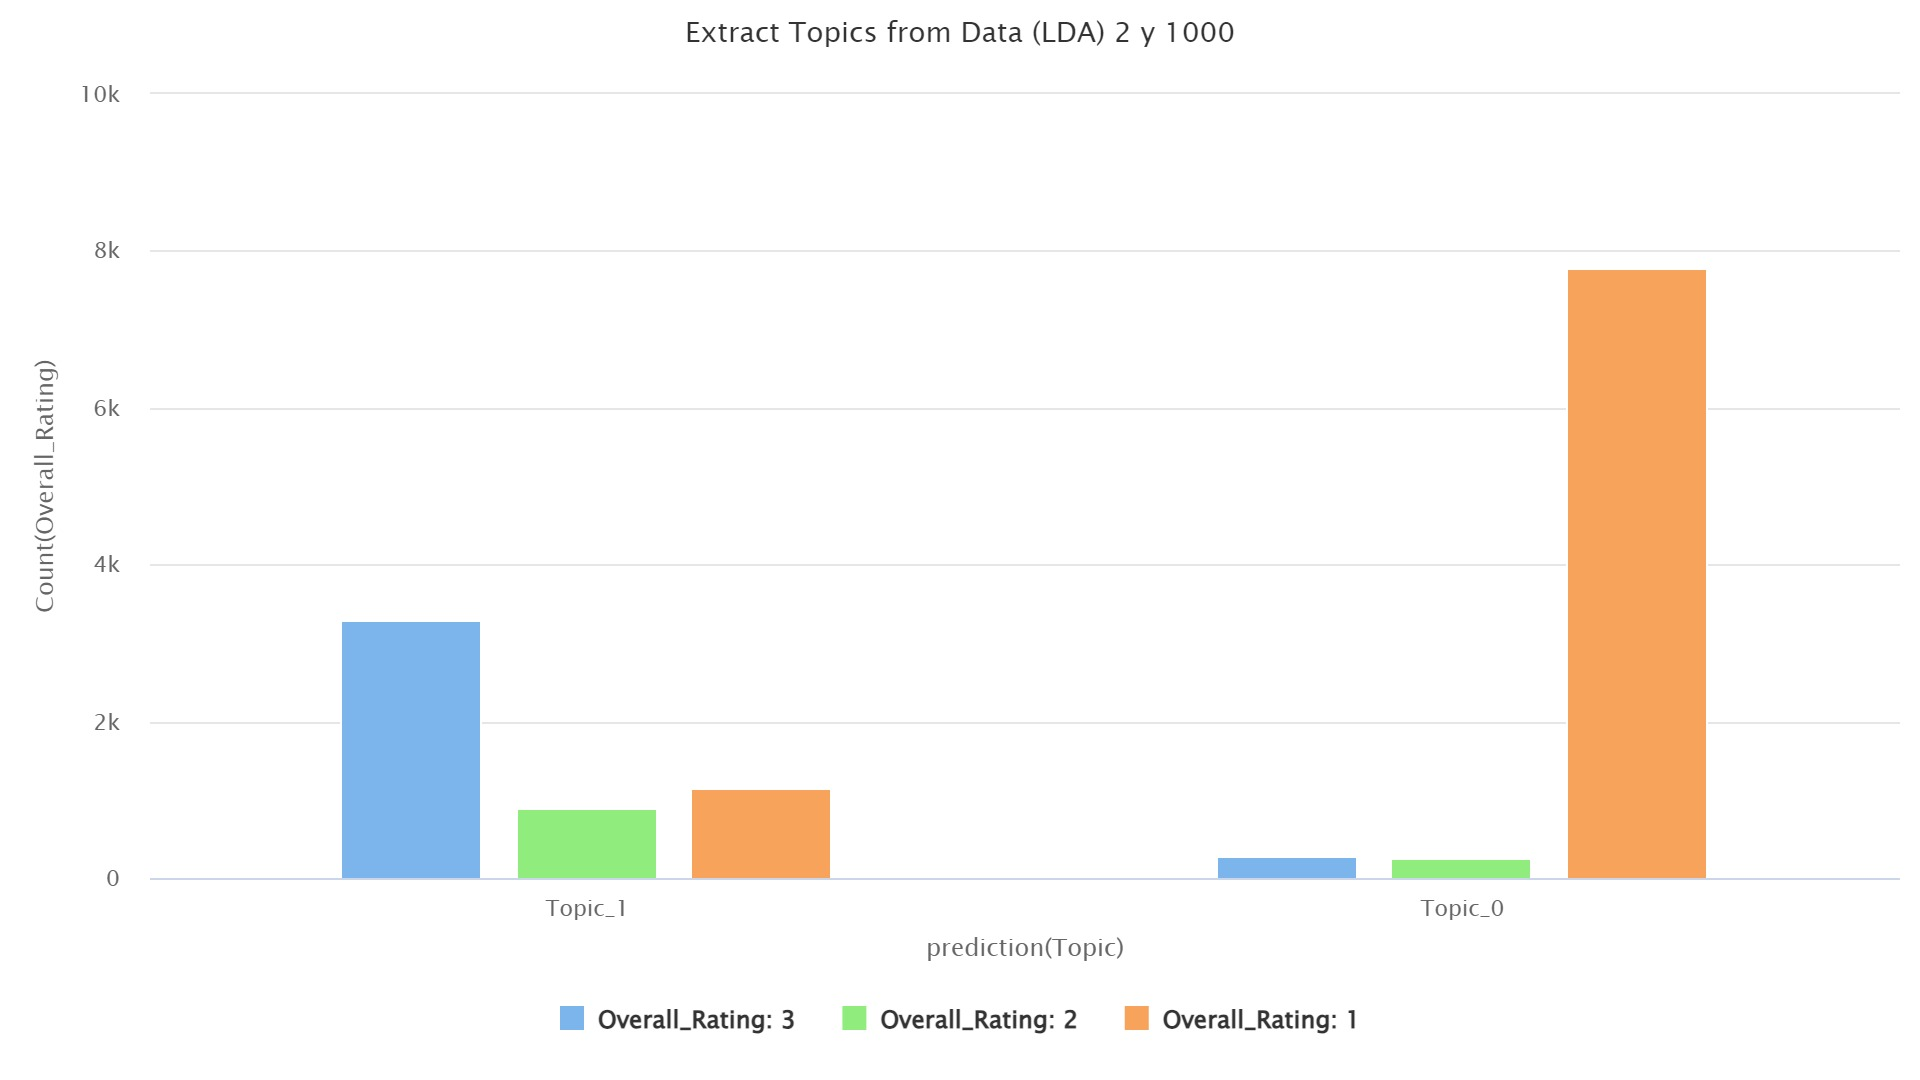
\includegraphics[width=0.85\linewidth]{graph_2topic_1000iter_rating.jpeg}\\
    \caption{Resultados de topic modelling basado en Overall\_Rating.}
\end{figure}

Se concluye que el método de \textit{topic modelling} en este caso puede resultar una
herramienta útil para la clasificación de instancias en dos grupos, existiendo
patrones en los datos que contribuyen a dos agrupaciones naturales de estos en
reseñas positivas y negativas.

\section{Conclusiones de la práctica}
\label{chap:conclusion}

Esta práctica nos ha permitido explorar nuevas técnicas para la construcción de
modelos. En concreto, hemos podido comprobar como el \textit{text mining} y el
\textit{análisis de sentimientos} son herramientas muy últiles capaces de
inferir información a partir de pocos campos textuales. Nos resulta
verdaderamente interesante comprobar como el campo de la inteligencia
artificial ha evolucionado hasta extremos donde es capaz de reconocer la
actitud de un agente hacia un dominio a través de una información tan compleja
como es el lenguaje natural.

También nos gustaría destacar como esta clase de herramientas deben usarse con
conocimiento ya que muchas presentan una gran complejidad que afecta
fuertemente al tiempo de entrenamiento y el rendimiento de los modelos. Esto
nos hace ver la importancia de un correcto entendimiento de las técnicas y
modelos empleados; destacando nuestro valor como ingenieros en el campo de la
Inteligencia Artificial.

  \end{report}


  % bibliography
  \phantomsection
  \addcontentsline{toc}{section}{Bibliografía}
  \label{bibliography}
  % \section{Bibliografía}
  \printbibliography[title={Bibliografía}]  % alternative

  % appendices
  % \begin{appendices}
  %   \part{Apéndices}  % optional
  %   \section{Mi apéndice}
  %   \lipsum[1]
  % \end{appendices}

\end{document}
